\chapter{Testy architektury \texttt{STP} \label{chap:testy_stp}}
Kolejnym etapem jakim poddano aplikację było przetestowanie zaimplementowanej warstwy wzorowanej na architekturze \texttt{STP}.
Każda zgłoszona do rozgrywek drużyna, przed przystąpieniem do turnieju głównego musi przejść eliminacje sprawdzające jej poziom.
Jako zadania testowe postanowiono wybrać niektóre rzeczywiste zadania elimincyjne, przez jakie musiały przejść drużyny w ostatnich latach.
Więcej informacji na temat eliminacji można znaleźć na stronie projektu \cite{robocup}.
\section{ Nawigacja w dynamicznym środowisku \label{sec:2011}}
Pierwszym zadanie pochodzi z eliminacji do mistrzostw w $2011$ roku.
Celem próby jest sprawdzenie zdolności robotów do bezpiecznego poruszania się w dynamicznym środowisku. Poniżej zamieszczono rysunek przedstawiający 
środowisko testowe. Znajduje się na nim 6 robotów pełniących role przeszkód. Dwa z pośród nich są nieruchome, a pozostałe cztery poruszają się wzdłuż
zaznaczonej linii prostej.
\begin{figure}[!h]
\centering
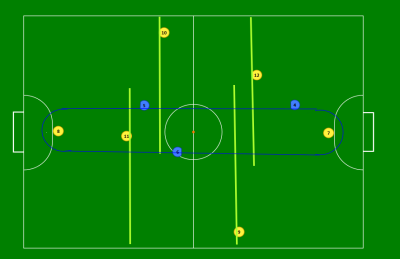
\includegraphics[scale=0.4]{./testy_stp/test_area_1}
\caption{Plan środowiska testowego} \label{fig:arch}
\end{figure}
Zasady eksperymentu są następujące:
\begin{enumerate}
\item Liczba startujących robotów jest ograniczona do trzech.
\item Uczestniczące roboty muszą poruszać się pomiędzy dwoma nieruchomymi przeszkodami.
\item Każdorazowo kiedy robot dotknie przeszkody otrzymuje punkt ujemny.
\item Każdy uczestnik, który pokona z powodzeniem trasę otrzymuje punkt.
\item Robot, który wykona okrążenie z piłką otrzymuje dodatkowo 2 punkty.
\item Test trwa 2 minuty.
\end{enumerate}

\subsection{ Wyniki testu nawigacji }
\subsubsection{Rezultaty uczestników eliminacji}

\section{ Strzelanie po podaniu }
Kolejne zadanie pochodzi z $2009$ roku. W zadaniu uczestniczy od $2$ do $3$ robotów z jednej drużyny. Ich zadaniem jest zdobycie jak największej ilości goli w przeciągu
$120$ sekund. Punkty przyznawane są następująco:
\begin{enumerate}
    \item  drużyna zdobywa 1 punkt w momencie gdy przed poprawnym strzałem na bramkę dwa roboty dotkną piłki ( wykonane zostanie np. jedno podanie).
    \item  drużyna zdobywa 2 punkty gdy przed oddanym strzałem $3$ roboty dotkną piłki.
\end{enumerate}

Zasady eksperymentu zamieszczono poniżej:
\begin{enumerate}
    \item  Przed startem wszytkie roboty muszą być umieszczone w odległości nie przekraczającej $1[m]$ od własnej linii bramkowej, 
    \item  Zawodnicy drużyny przeciwnej pełnią rolę statycznych przeszkód,
    \item  Przy każdym starcie piłka jest umieszczana w jedynm z narożników, na własnej połowie grającej drużyny,
    \item  Gol może być zdobyty tylko w sytuacji, gdy robot znajdduje się na połowie przeciwnika,
    \item  Po zdobytej bramce piłka ponownie wraca do jednego z narożników.
\end{enumerate}

\subsection{ Wyniki testu }
\subsubsection{Rezultaty uczestników eliminacji}